% Options for packages loaded elsewhere
\PassOptionsToPackage{unicode}{hyperref}
\PassOptionsToPackage{hyphens}{url}
%
\documentclass[
]{article}
\usepackage{amsmath,amssymb}
\usepackage{iftex}
\ifPDFTeX
  \usepackage[T1]{fontenc}
  \usepackage[utf8]{inputenc}
  \usepackage{textcomp} % provide euro and other symbols
\else % if luatex or xetex
  \usepackage{unicode-math} % this also loads fontspec
  \defaultfontfeatures{Scale=MatchLowercase}
  \defaultfontfeatures[\rmfamily]{Ligatures=TeX,Scale=1}
\fi
\usepackage{lmodern}
\ifPDFTeX\else
  % xetex/luatex font selection
\fi
% Use upquote if available, for straight quotes in verbatim environments
\IfFileExists{upquote.sty}{\usepackage{upquote}}{}
\IfFileExists{microtype.sty}{% use microtype if available
  \usepackage[]{microtype}
  \UseMicrotypeSet[protrusion]{basicmath} % disable protrusion for tt fonts
}{}
\makeatletter
\@ifundefined{KOMAClassName}{% if non-KOMA class
  \IfFileExists{parskip.sty}{%
    \usepackage{parskip}
  }{% else
    \setlength{\parindent}{0pt}
    \setlength{\parskip}{6pt plus 2pt minus 1pt}}
}{% if KOMA class
  \KOMAoptions{parskip=half}}
\makeatother
\usepackage{xcolor}
\usepackage[margin=1in]{geometry}
\usepackage{longtable,booktabs,array}
\usepackage{calc} % for calculating minipage widths
% Correct order of tables after \paragraph or \subparagraph
\usepackage{etoolbox}
\makeatletter
\patchcmd\longtable{\par}{\if@noskipsec\mbox{}\fi\par}{}{}
\makeatother
% Allow footnotes in longtable head/foot
\IfFileExists{footnotehyper.sty}{\usepackage{footnotehyper}}{\usepackage{footnote}}
\makesavenoteenv{longtable}
\usepackage{graphicx}
\makeatletter
\def\maxwidth{\ifdim\Gin@nat@width>\linewidth\linewidth\else\Gin@nat@width\fi}
\def\maxheight{\ifdim\Gin@nat@height>\textheight\textheight\else\Gin@nat@height\fi}
\makeatother
% Scale images if necessary, so that they will not overflow the page
% margins by default, and it is still possible to overwrite the defaults
% using explicit options in \includegraphics[width, height, ...]{}
\setkeys{Gin}{width=\maxwidth,height=\maxheight,keepaspectratio}
% Set default figure placement to htbp
\makeatletter
\def\fps@figure{htbp}
\makeatother
\setlength{\emergencystretch}{3em} % prevent overfull lines
\providecommand{\tightlist}{%
  \setlength{\itemsep}{0pt}\setlength{\parskip}{0pt}}
\setcounter{secnumdepth}{-\maxdimen} % remove section numbering
% Use this file as a preamble to create pdf's with dfSummaries.
% One possible way if to use it directly in the YAML section:
% output: 
%   pdf_document: 
%     latex_engine: xelatex
%     includes:
%       in_header: 
%       - !expr system.file("includes/fig-valign.tex", package = "summarytools")
\usepackage{graphicx}
\usepackage[export]{adjustbox}
\usepackage{letltxmacro}
\LetLtxMacro{\OldIncludegraphics}{\includegraphics}
\renewcommand{\includegraphics}[2][]{\raisebox{0.5\height}%
  {\OldIncludegraphics[valign=t,#1]{#2}}}
\ifLuaTeX
  \usepackage{selnolig}  % disable illegal ligatures
\fi
\IfFileExists{bookmark.sty}{\usepackage{bookmark}}{\usepackage{hyperref}}
\IfFileExists{xurl.sty}{\usepackage{xurl}}{} % add URL line breaks if available
\urlstyle{same}
\hypersetup{
  pdftitle={Análise de Mortalidade por Causas Externas},
  pdfauthor={Samuel Martins de Medeiros},
  hidelinks,
  pdfcreator={LaTeX via pandoc}}

\title{Análise de Mortalidade por Causas Externas}
\author{Samuel Martins de Medeiros}
\date{}

\begin{document}
\maketitle

\hypertarget{conjunto-de-dados-e-problema-apresentado.}{%
\subsection{Conjunto de Dados e Problema
Apresentado.}\label{conjunto-de-dados-e-problema-apresentado.}}

Tendo como objetivo investigar as tendências de mortalidade no Capítulo
XX do CID-10 ao longo do período de 2012 a 2020, busca-se identificar
grupos mais suscetíveis a homicídios ou suicídios com base em variáveis
demográficas, como sexo, faixa etária, escolaridade, UF de residência,
estado civil e raça/cor através de análises descritivas realizadas no
relatório. Também será realizada uma análise das CIDs (Classificação
Internacional de Doenças) ao longo dos anos investigados.

Para realizar esta análise estatística, utilizaremos o conjunto de dados
proveniente do Sistema de Informações sobre Mortalidade (SIM), com uma
restrição específica. O conjunto de dados será limitado às informações
referentes a gestantes e puérperas, bem como ao grupo de mulheres em
período fértil. As análises a priori foram realizadas de forma separada
para os dois bancos, com uma amostra de 3294 (gestantes e puérperas) e
128899 (Mulheres em período fértil).

Dessa forma, o estudo terá como foco a compreensão das tendências de
mortalidade relacionadas a homicídios, suicídios, acidentes e outros
nesses grupos específicos. Essa restrição nos permitirá direcionar
nossas análises e explorar possíveis diferenças nas taxas de mortalidade
entre mulheres gestantes, puérperas e não gestantes em futuros
realatorios, com o objetivo de identificar grupos mais sensíveis a essas
causas específicas de morte ao longo dos anos.

\hypertarget{panorama-geral-de-mortalidade-materna-por-causas-externas-no-brasil}{%
\subsection{Panorama geral de mortalidade materna por causas externas no
Brasil}\label{panorama-geral-de-mortalidade-materna-por-causas-externas-no-brasil}}

Antes de iniciarmos a investigação das tendências recentes e dos níveis
gerais de mortalidade, é importante observar, por meio da Tabela 1, que
nosso conjunto de dados apresenta informações inconsistentes em relação
ao sexo. Nossas restrições indicam que os valores devem ser
exclusivamente `F' (feminino), no entanto, foram identificados registros
com valores diferentes. Ambos dados implausíveis são apresentados para o
banco de dados de gestantes e puérperas.

Além disso, encontramos também dados questionáveis relacionados à idade.
Para gestantes e puérperas, notamos a presença de valores de idade
menores que 10 ou superiores a 55. Ainda sim os dados serão considerados
na análise.

\begin{longtable}[]{@{}
  >{\raggedright\arraybackslash}p{(\columnwidth - 8\tabcolsep) * \real{0.1286}}
  >{\raggedright\arraybackslash}p{(\columnwidth - 8\tabcolsep) * \real{0.3714}}
  >{\raggedleft\arraybackslash}p{(\columnwidth - 8\tabcolsep) * \real{0.2429}}
  >{\raggedright\arraybackslash}p{(\columnwidth - 8\tabcolsep) * \real{0.1714}}
  >{\raggedleft\arraybackslash}p{(\columnwidth - 8\tabcolsep) * \real{0.0857}}@{}}
\caption{Dados Implausíveis}\tabularnewline
\toprule\noalign{}
\begin{minipage}[b]{\linewidth}\raggedright
Variavel
\end{minipage} & \begin{minipage}[b]{\linewidth}\raggedright
Valor
\end{minipage} & \begin{minipage}[b]{\linewidth}\raggedleft
Qtd.Implausiveis
\end{minipage} & \begin{minipage}[b]{\linewidth}\raggedright
Porcentagem
\end{minipage} & \begin{minipage}[b]{\linewidth}\raggedleft
Total
\end{minipage} \\
\midrule\noalign{}
\endfirsthead
\toprule\noalign{}
\begin{minipage}[b]{\linewidth}\raggedright
Variavel
\end{minipage} & \begin{minipage}[b]{\linewidth}\raggedright
Valor
\end{minipage} & \begin{minipage}[b]{\linewidth}\raggedleft
Qtd.Implausiveis
\end{minipage} & \begin{minipage}[b]{\linewidth}\raggedright
Porcentagem
\end{minipage} & \begin{minipage}[b]{\linewidth}\raggedleft
Total
\end{minipage} \\
\midrule\noalign{}
\endhead
\bottomrule\noalign{}
\endlastfoot
Sexo & Valores diferentes de `F' & 3 & 0.091\% & 3294 \\
Idade & Idade \textless{} 10 ou Idade \textgreater{} 55 & 66 & 2.003\% &
3294 \\
\end{longtable}

\hypertarget{gestantes-e-puuxe9rperas.}{%
\subsubsection{Gestantes e Puérperas.}\label{gestantes-e-puuxe9rperas.}}

De início é possível observar, pela Tabela 2, a frequência de
observações para as variáveis consideradas no estudo, sendo elas as de
caracterização: Sexo, Raça/Cor, Escolaridade, Estado Civil e Faixa
Etária, e as variáveis de estudo Ano do obito e CID`s.

\hypertarget{table}{%
\subsubsection{Table}\label{table}}

\textbf{Dados}\\
\textbf{Dimensões:} 3294 x 7\\
\textbf{Duplicadas:} 1310

\begin{longtable}[]{@{}
  >{\raggedright\arraybackslash}p{(\columnwidth - 10\tabcolsep) * \real{0.0446}}
  >{\raggedright\arraybackslash}p{(\columnwidth - 10\tabcolsep) * \real{0.1429}}
  >{\raggedright\arraybackslash}p{(\columnwidth - 10\tabcolsep) * \real{0.2946}}
  >{\raggedright\arraybackslash}p{(\columnwidth - 10\tabcolsep) * \real{0.1696}}
  >{\raggedright\arraybackslash}p{(\columnwidth - 10\tabcolsep) * \real{0.2054}}
  >{\raggedright\arraybackslash}p{(\columnwidth - 10\tabcolsep) * \real{0.1071}}@{}}
\toprule\noalign{}
\begin{minipage}[b]{\linewidth}\raggedright
No
\end{minipage} & \begin{minipage}[b]{\linewidth}\raggedright
Variáveis
\end{minipage} & \begin{minipage}[b]{\linewidth}\raggedright
Estatísticas/Valores
\end{minipage} & \begin{minipage}[b]{\linewidth}\raggedright
Freq. De Válidos
\end{minipage} & \begin{minipage}[b]{\linewidth}\raggedright
Gráficos
\end{minipage} & \begin{minipage}[b]{\linewidth}\raggedright
Faltantes
\end{minipage} \\
\midrule\noalign{}
\endhead
\bottomrule\noalign{}
\endlastfoot
1 & \begin{minipage}[t]{\linewidth}\raggedright
sexo\\
{[}character{]}\strut
\end{minipage} & \begin{minipage}[t]{\linewidth}\raggedright
1. Feminino\\
2. Ignorado\\
3. Masculino\strut
\end{minipage} & \begin{minipage}[t]{\linewidth}\raggedright
3291 (99.9\%)\\
2 ( 0.1\%)\\
1 ( 0.0\%)\strut
\end{minipage} & \includegraphics{/tmp/ds0082.png} &
\begin{minipage}[t]{\linewidth}\raggedright
0\\
(0.0\%)\strut
\end{minipage} \\
2 & \begin{minipage}[t]{\linewidth}\raggedright
Raça/Cor\\
{[}character{]}\strut
\end{minipage} & \begin{minipage}[t]{\linewidth}\raggedright
1. Amarela\\
2. Branca\\
3. Ignorado\\
4. Indígena\\
5. Parda\\
6. Preta\strut
\end{minipage} & \begin{minipage}[t]{\linewidth}\raggedright
2 ( 0.1\%)\\
1201 (36.5\%)\\
82 ( 2.5\%)\\
37 ( 1.1\%)\\
1718 (52.2\%)\\
254 ( 7.7\%)\strut
\end{minipage} & \includegraphics{/tmp/ds0083.png} &
\begin{minipage}[t]{\linewidth}\raggedright
0\\
(0.0\%)\strut
\end{minipage} \\
3 & \begin{minipage}[t]{\linewidth}\raggedright
Escolaridade\\
{[}character{]}\strut
\end{minipage} & \begin{minipage}[t]{\linewidth}\raggedright
1. Fundamental I\\
2. Fundamental II\\
3. Ignorado\\
4. Médio\\
5. Não informado\\
6. Sem escolaridade\\
7. Superior completo\\
8. Superior incompleto\strut
\end{minipage} & \begin{minipage}[t]{\linewidth}\raggedright
400 (12.1\%)\\
1005 (30.5\%)\\
345 (10.5\%)\\
663 (20.1\%)\\
616 (18.7\%)\\
41 ( 1.2\%)\\
151 ( 4.6\%)\\
73 ( 2.2\%)\strut
\end{minipage} & \includegraphics{/tmp/ds0084.png} &
\begin{minipage}[t]{\linewidth}\raggedright
0\\
(0.0\%)\strut
\end{minipage} \\
4 & \begin{minipage}[t]{\linewidth}\raggedright
Estado Civil\\
{[}character{]}\strut
\end{minipage} & \begin{minipage}[t]{\linewidth}\raggedright
1. Casado\\
2. Ignorado\\
3. Separado Judic./Divorciad\\
4. Solteiro\\
5. Viúvo\strut
\end{minipage} & \begin{minipage}[t]{\linewidth}\raggedright
476 (14.5\%)\\
601 (18.2\%)\\
64 ( 1.9\%)\\
2137 (64.9\%)\\
16 ( 0.5\%)\strut
\end{minipage} & \includegraphics{/tmp/ds0085.png} &
\begin{minipage}[t]{\linewidth}\raggedright
0\\
(0.0\%)\strut
\end{minipage} \\
5 & \begin{minipage}[t]{\linewidth}\raggedright
Faixa Etaria\\
{[}character{]}\strut
\end{minipage} & \begin{minipage}[t]{\linewidth}\raggedright
1. até 10 anos\\
2. De 11 a 15 anos\\
3. De 16 a 19 anos\\
4. De 20 a 29 anos\\
5. De 30 a 39 anos\\
6. De 40 a 50 anos\\
7. Mais de 50 anos\\
8. Não informado\strut
\end{minipage} & \begin{minipage}[t]{\linewidth}\raggedright
28 ( 0.9\%)\\
84 ( 2.6\%)\\
559 (17.0\%)\\
1581 (48.0\%)\\
788 (23.9\%)\\
184 ( 5.6\%)\\
48 ( 1.5\%)\\
22 ( 0.7\%)\strut
\end{minipage} & \includegraphics{/tmp/ds0086.png} &
\begin{minipage}[t]{\linewidth}\raggedright
0\\
(0.0\%)\strut
\end{minipage} \\
6 & \begin{minipage}[t]{\linewidth}\raggedright
CID\\
{[}character{]}\strut
\end{minipage} & \begin{minipage}[t]{\linewidth}\raggedright
1. Acidentes automobilístico\\
2. Acidentes Envenenamento a\\
3. Acidentes Eventos ambient\\
4. Acidentes Quedas/afogamen\\
5. Homicídio\\
6. Outro\\
7. Suicídio\strut
\end{minipage} & \begin{minipage}[t]{\linewidth}\raggedright
1023 (31.1\%)\\
147 ( 4.5\%)\\
48 ( 1.5\%)\\
171 ( 5.2\%)\\
1308 (39.7\%)\\
214 ( 6.5\%)\\
383 (11.6\%)\strut
\end{minipage} & \includegraphics{/tmp/ds0087.png} &
\begin{minipage}[t]{\linewidth}\raggedright
0\\
(0.0\%)\strut
\end{minipage} \\
7 & \begin{minipage}[t]{\linewidth}\raggedright
Ano do Obito\\
{[}factor{]}\strut
\end{minipage} & \begin{minipage}[t]{\linewidth}\raggedright
1. 2011\\
2. 2012\\
3. 2013\\
4. 2014\\
5. 2015\\
6. 2016\\
7. 2017\\
8. 2018\\
9. 2019\\
10. 2020\strut
\end{minipage} & \begin{minipage}[t]{\linewidth}\raggedright
373 (11.3\%)\\
382 (11.6\%)\\
324 ( 9.8\%)\\
307 ( 9.3\%)\\
350 (10.6\%)\\
318 ( 9.7\%)\\
344 (10.4\%)\\
321 ( 9.7\%)\\
299 ( 9.1\%)\\
276 ( 8.4\%)\strut
\end{minipage} & \includegraphics{/tmp/ds0088.png} &
\begin{minipage}[t]{\linewidth}\raggedright
0\\
(0.0\%)\strut
\end{minipage} \\
\end{longtable}

Para maior facilidade de entendimento, é apresentado na Figura 1, o
desenvolvimento do número de casos de morte no decorrer dos anos para
entendimento de seu comportamento.

\begin{figure}
\centering
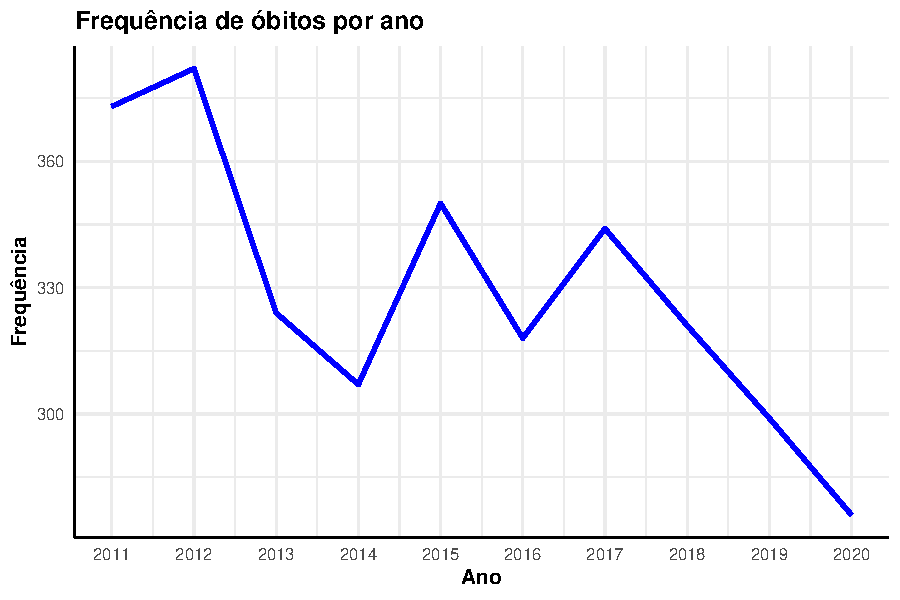
\includegraphics{RelatorioV03_files/figure-latex/unnamed-chunk-2-1.pdf}
\caption{Frequência de obitos por ano grupo Gestantes e Puérperas}
\end{figure}

Perceba que é apresentado um padrão de decrescimento no decorrer dos
anos. É de imporância para nossa análise a verificação de frequência de
morte por período gestaccional ou puerpério que ocorre o óbito, como
verificado na Tabela 3, onde valores faltantes foram assumidos como `Não
Informados'.

\begin{longtable}[]{@{}lrr@{}}
\caption{Período do Óbito}\tabularnewline
\toprule\noalign{}
& n & \% \\
\midrule\noalign{}
\endfirsthead
\toprule\noalign{}
& n & \% \\
\midrule\noalign{}
\endhead
\bottomrule\noalign{}
\endlastfoot
Até 42 dias após o parto & 223 & 6.8 \\
De 43 dias a 1 ano após o parto & 1007 & 30.6 \\
Na gravidez & 1522 & 46.2 \\
Não Informado & 412 & 12.5 \\
No aborto & 18 & 0.5 \\
No parto & 112 & 3.4 \\
Total & 3294 & 100.0 \\
\end{longtable}

\hypertarget{mulheres-em-peruxedodo-fuxe9rtil.}{%
\subsubsection{Mulheres em Período
Fértil.}\label{mulheres-em-peruxedodo-fuxe9rtil.}}

Todas as análises apresentadas para os tópicos em estudo serão
replicadas para os grupos de Mulheres em Período Fértil. Como
apresentado na Tabela 4, temos a representação da distribuição de
frequência dos dados bem como respectivas porcentagens.

\begin{longtable}[]{@{}
  >{\raggedright\arraybackslash}p{(\columnwidth - 2\tabcolsep) * \real{0.7639}}
  >{\centering\arraybackslash}p{(\columnwidth - 2\tabcolsep) * \real{0.2361}}@{}}
\caption{Frequência por variável para o grupo Mulheres em Período
Fértil}\tabularnewline
\toprule\noalign{}
\begin{minipage}[b]{\linewidth}\raggedright
\textbf{Characteristic}
\end{minipage} & \begin{minipage}[b]{\linewidth}\centering
\textbf{N = 128,899}
\end{minipage} \\
\midrule\noalign{}
\endfirsthead
\toprule\noalign{}
\begin{minipage}[b]{\linewidth}\raggedright
\textbf{Characteristic}
\end{minipage} & \begin{minipage}[b]{\linewidth}\centering
\textbf{N = 128,899}
\end{minipage} \\
\midrule\noalign{}
\endhead
\bottomrule\noalign{}
\endlastfoot
\textbf{sexo} & \\
Feminino & 128,899 (100\%) \\
\textbf{Raça/Cor} & \\
Amarela & 294 (0.2\%) \\
Branca & 52,505 (41\%) \\
Ignorado & 3,856 (3.0\%) \\
Indígena & 804 (0.6\%) \\
Parda & 63,609 (49\%) \\
Preta & 7,831 (6.1\%) \\
\textbf{Escolaridade} & \\
Fundamental I & 17,473 (14\%) \\
Fundamental II & 31,502 (24\%) \\
Ignorado & 15,147 (12\%) \\
Médio & 25,766 (20\%) \\
Não informado & 23,718 (18\%) \\
Sem escolaridade & 3,442 (2.7\%) \\
Superior completo & 7,660 (5.9\%) \\
Superior incompleto & 4,191 (3.3\%) \\
\textbf{Estado Civil} & \\
Casado & 24,281 (19\%) \\
Ignorado & 17,493 (14\%) \\
Separado Judic./Divorciado & 7,047 (5.5\%) \\
Solteiro & 77,522 (60\%) \\
Viúvo & 2,556 (2.0\%) \\
\textbf{Faixa Etaria} & \\
até 10 anos & 362 (0.3\%) \\
De 11 a 15 anos & 6,487 (5.0\%) \\
De 16 a 19 anos & 12,470 (9.7\%) \\
De 20 a 29 anos & 33,821 (26\%) \\
De 30 a 39 anos & 31,872 (25\%) \\
De 40 a 50 anos & 30,000 (23\%) \\
Mais de 50 anos & 13,318 (10\%) \\
Não informado & 569 (0.4\%) \\
\textbf{CID} & \\
Acidentes automobilísticos & 44,761 (35\%) \\
Acidentes Envenenamento acidental & 2,828 (2.2\%) \\
Acidentes Eventos ambientais & 1,954 (1.5\%) \\
Acidentes Quedas/afogamento/inalação/corrente elétrica & 10,389
(8.1\%) \\
Homicídio & 37,567 (29\%) \\
Outro & 12,139 (9.4\%) \\
Suicídio & 19,261 (15\%) \\
\textbf{Ano do Obito} & \\
2011 & 13,533 (10\%) \\
2012 & 13,801 (11\%) \\
2013 & 13,396 (10\%) \\
2014 & 13,690 (11\%) \\
2015 & 12,735 (9.9\%) \\
2016 & 12,676 (9.8\%) \\
2017 & 12,984 (10\%) \\
2018 & 12,166 (9.4\%) \\
2019 & 11,838 (9.2\%) \\
2020 & 12,080 (9.4\%) \\
\end{longtable}

Na Figura 2 vemos a representação da evolução do número de casos de
óbito notificados para o grupo em questão.

\begin{figure}
\centering
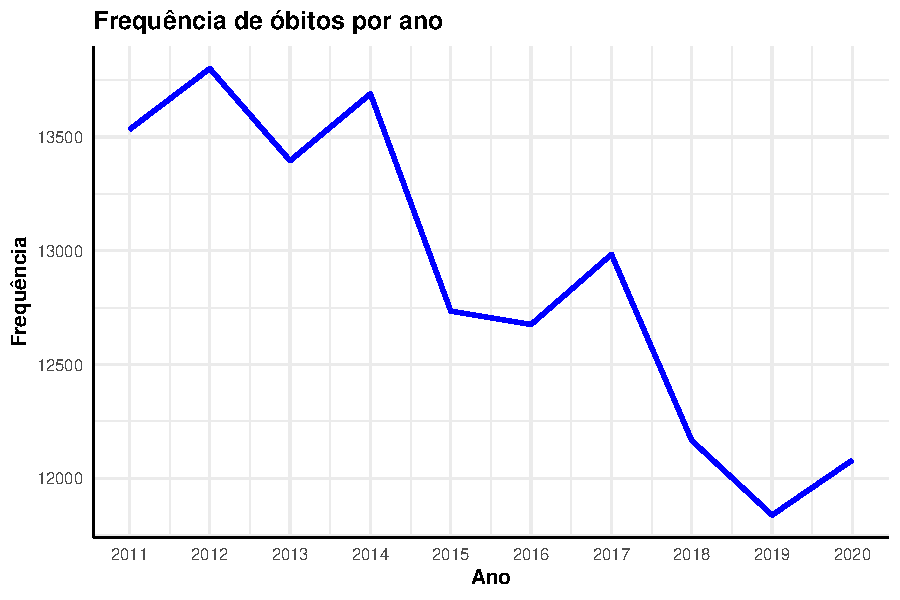
\includegraphics{RelatorioV03_files/figure-latex/unnamed-chunk-5-1.pdf}
\caption{Frequência de obitos por ano grupo Mulheres em Período Fértil}
\end{figure}

Ao contrário do grupo anterior, os dados apresentam um crescimento do
penúltimo para último ano.

\hypertarget{tenduxeancia-nos-uxfaltimos-anos-nas-taxas-de-acidente-suicuxeddio-e-homicuxeddio.}{%
\subsection{Tendência nos últimos anos nas taxas de acidente, suicídio e
homicídio.}\label{tenduxeancia-nos-uxfaltimos-anos-nas-taxas-de-acidente-suicuxeddio-e-homicuxeddio.}}

\hypertarget{gestantes-e-puerperas.}{%
\subsubsection{Gestantes e Puerperas.}\label{gestantes-e-puerperas.}}

Para discutir a respeito dessa hipótese, seguindo com a análise
apresentada no tópico anterior, é apresentado na Figura 3, a evolução do
número de casos separado por: Acidentes de forma geral, Homicídio,
Suicídio e Outros para os dados de Gestantes e Puerperas.

\begin{figure}
\centering
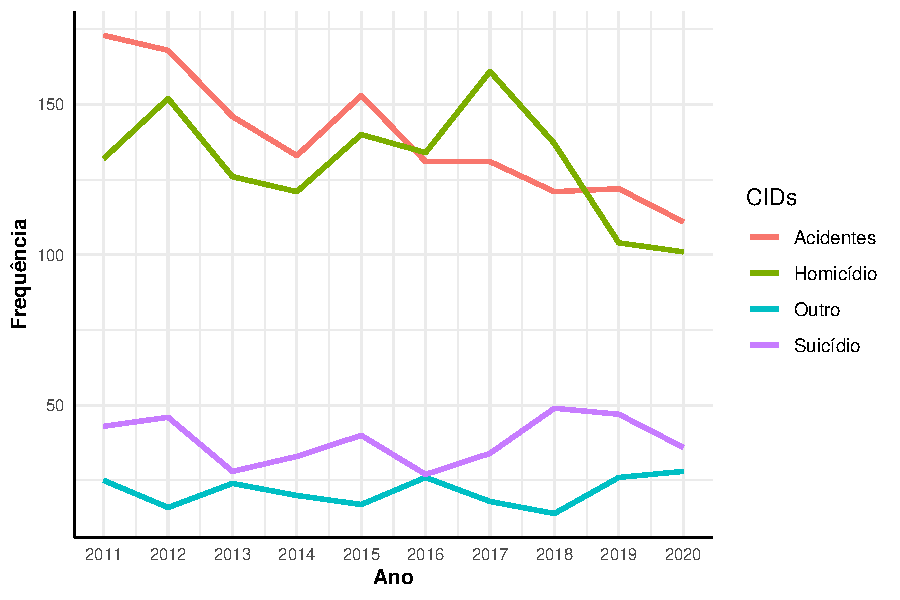
\includegraphics{RelatorioV03_files/figure-latex/unnamed-chunk-6-1.pdf}
\caption{Frequência de Obitos por CID para Gestantes e Puérperas}
\end{figure}

Apresentando um descresimo para Homicidios e Acidentes e uma
estabilidade para Suicidio e Outras causas. Pode-se visuaizar esses
dados melhor através da Tabela 5.

\begin{longtable}[]{@{}rllll@{}}
\caption{Porcentagem de CID por Ano para Gestantes e
Puerperas}\tabularnewline
\toprule\noalign{}
Ano & Acidentes & Homicídio & Outro & Suicídio \\
\midrule\noalign{}
\endfirsthead
\toprule\noalign{}
Ano & Acidentes & Homicídio & Outro & Suicídio \\
\midrule\noalign{}
\endhead
\bottomrule\noalign{}
\endlastfoot
2011 & 46.38\% & 35.39\% & 6.70\% & 11.53\% \\
2012 & 43.98\% & 39.79\% & 4.19\% & 12.04\% \\
2013 & 45.06\% & 38.89\% & 7.41\% & 8.64\% \\
2014 & 43.32\% & 39.41\% & 6.51\% & 10.75\% \\
2015 & 43.71\% & 40.00\% & 4.86\% & 11.43\% \\
2016 & 41.19\% & 42.14\% & 8.18\% & 8.49\% \\
2017 & 38.08\% & 46.80\% & 5.23\% & 9.88\% \\
2018 & 37.69\% & 42.68\% & 4.36\% & 15.26\% \\
2019 & 40.80\% & 34.78\% & 8.70\% & 15.72\% \\
2020 & 40.22\% & 36.59\% & 10.14\% & 13.04\% \\
\end{longtable}

As taxas de Acidentes, seguidas pelas de Homicídio, permanecem as
maiores em todos os anos, com exceção de 2016 e de 2018 a 2020 onde a
afirmação é invertida e Homicídio passa a ser maior que Acidentes.

\hypertarget{mulheres-em-peruxedodo-fuxe9rtil}{%
\subsubsection{Mulheres em Período
Fértil}\label{mulheres-em-peruxedodo-fuxe9rtil}}

Seguindo com a análise, na Figura 4 é apresentado os dados de CID por
ano para o grupo de Mulheres em período Fértil. Diferentemente do grupo
de Gestantes aqui as causasa apresentam-se mais bem retratadas para os
anos, onde vemos Acidentes com maior valor seguido por Homicidio,
apresentando um descrescimento enquanto Suicídios e Outras causas
apresentam um crescimento.

\begin{figure}
\centering
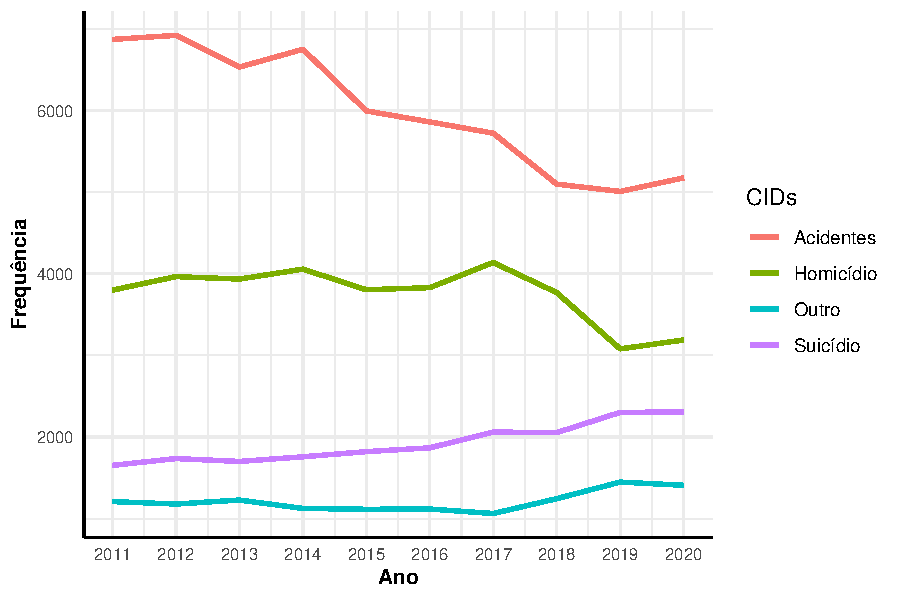
\includegraphics{RelatorioV03_files/figure-latex/unnamed-chunk-8-1.pdf}
\caption{Frequência de Obitos por CID para Mulheres em Período Fértil}
\end{figure}

Na Tabela 6 é possível ver retratado as porcentagens respectivas a cada
causa por cada ano, onde vemos as afirmações ateriores.

\begin{longtable}[]{@{}rllll@{}}
\caption{Porcentagem de CID por Ano para Mulheres em Período
Fértil}\tabularnewline
\toprule\noalign{}
Ano & Acidentes & Homicídio & Outro & Suicídio \\
\midrule\noalign{}
\endfirsthead
\toprule\noalign{}
Ano & Acidentes & Homicídio & Outro & Suicídio \\
\midrule\noalign{}
\endhead
\bottomrule\noalign{}
\endlastfoot
2011 & 50.77\% & 28.08\% & 8.93\% & 12.21\% \\
2012 & 50.15\% & 28.73\% & 8.54\% & 12.58\% \\
2013 & 48.76\% & 29.37\% & 9.17\% & 12.70\% \\
2014 & 49.31\% & 29.63\% & 8.22\% & 12.84\% \\
2015 & 47.07\% & 29.87\% & 8.76\% & 14.30\% \\
2016 & 46.23\% & 30.21\% & 8.82\% & 14.74\% \\
2017 & 44.07\% & 31.87\% & 8.19\% & 15.87\% \\
2018 & 41.90\% & 30.98\% & 10.23\% & 16.88\% \\
2019 & 42.30\% & 26.02\% & 12.23\% & 19.45\% \\
2020 & 42.84\% & 26.40\% & 11.66\% & 19.10\% \\
\end{longtable}

\hypertarget{anuxe1lise-de-vulnerabilidade-dos-peruxedodos-de-gestauxe7uxe3o}{%
\subsection{Análise de vulnerabilidade dos períodos de
gestação}\label{anuxe1lise-de-vulnerabilidade-dos-peruxedodos-de-gestauxe7uxe3o}}

Aqui será considerado apenas o grupo de Gestantes e Puérperas para
análise, considerando o tema do tópico.

Foi realizado testes de independência usando o teste Qui-Quadrado e o
teste exato de Fisher (quando houver falta de observações para o
Qui-Quadrado) afim de identificar se há algum tipo de relação entre as
variáveis período gestacional ou puérperio do óbito com a variável
Homicídio e Suicídio. Esses dados são apresentados na Tabela 7 e Tabela
8 para Suicídio e Homicídio respectivamente. Assumindo a hipótese de
independência como hipótese nula, rejeitamos para ambas as variáveis, a
um \(\alpha = 0.05\), nos levando a crer que existe sim um período
gestacional mais vulnerável.

\begin{longtable}[]{@{}
  >{\raggedright\arraybackslash}p{(\columnwidth - 16\tabcolsep) * \real{0.0861}}
  >{\centering\arraybackslash}p{(\columnwidth - 16\tabcolsep) * \real{0.1722}}
  >{\centering\arraybackslash}p{(\columnwidth - 16\tabcolsep) * \real{0.2185}}
  >{\centering\arraybackslash}p{(\columnwidth - 16\tabcolsep) * \real{0.0927}}
  >{\centering\arraybackslash}p{(\columnwidth - 16\tabcolsep) * \real{0.0993}}
  >{\centering\arraybackslash}p{(\columnwidth - 16\tabcolsep) * \real{0.0728}}
  >{\centering\arraybackslash}p{(\columnwidth - 16\tabcolsep) * \real{0.0795}}
  >{\centering\arraybackslash}p{(\columnwidth - 16\tabcolsep) * \real{0.0927}}
  >{\centering\arraybackslash}p{(\columnwidth - 16\tabcolsep) * \real{0.0861}}@{}}
\caption{Teste para Suicídio}\tabularnewline
\toprule\noalign{}
\begin{minipage}[b]{\linewidth}\raggedright
\end{minipage} & \begin{minipage}[b]{\linewidth}\centering
Até 42 dias após o parto
\end{minipage} & \begin{minipage}[b]{\linewidth}\centering
De 43 dias a 1 ano após o parto
\end{minipage} & \begin{minipage}[b]{\linewidth}\centering
Na gravidez
\end{minipage} & \begin{minipage}[b]{\linewidth}\centering
Nao Informado
\end{minipage} & \begin{minipage}[b]{\linewidth}\centering
No aborto
\end{minipage} & \begin{minipage}[b]{\linewidth}\centering
No parto
\end{minipage} & \begin{minipage}[b]{\linewidth}\centering
\textbf{Total}
\end{minipage} & \begin{minipage}[b]{\linewidth}\centering
\textbf{p-value}
\end{minipage} \\
\midrule\noalign{}
\endfirsthead
\toprule\noalign{}
\begin{minipage}[b]{\linewidth}\raggedright
\end{minipage} & \begin{minipage}[b]{\linewidth}\centering
Até 42 dias após o parto
\end{minipage} & \begin{minipage}[b]{\linewidth}\centering
De 43 dias a 1 ano após o parto
\end{minipage} & \begin{minipage}[b]{\linewidth}\centering
Na gravidez
\end{minipage} & \begin{minipage}[b]{\linewidth}\centering
Nao Informado
\end{minipage} & \begin{minipage}[b]{\linewidth}\centering
No aborto
\end{minipage} & \begin{minipage}[b]{\linewidth}\centering
No parto
\end{minipage} & \begin{minipage}[b]{\linewidth}\centering
\textbf{Total}
\end{minipage} & \begin{minipage}[b]{\linewidth}\centering
\textbf{p-value}
\end{minipage} \\
\midrule\noalign{}
\endhead
\bottomrule\noalign{}
\endlastfoot
\textbf{Suicidio} & & & & & & & & 0.005 \\
Não & 191 (86\%) & 871 (86\%) & 1,377 (90\%) & 362 (88\%) & 13 (72\%) &
97 (87\%) & 2,911 (88\%) & \\
Sim & 32 (14\%) & 136 (14\%) & 145 (9.5\%) & 50 (12\%) & 5 (28\%) & 15
(13\%) & 383 (12\%) & \\
\textbf{Total} & 223 (100\%) & 1,007 (100\%) & 1,522 (100\%) & 412
(100\%) & 18 (100\%) & 112 (100\%) & 3,294 (100\%) & \\
\end{longtable}

\begin{longtable}[]{@{}
  >{\raggedright\arraybackslash}p{(\columnwidth - 16\tabcolsep) * \real{0.0921}}
  >{\centering\arraybackslash}p{(\columnwidth - 16\tabcolsep) * \real{0.1711}}
  >{\centering\arraybackslash}p{(\columnwidth - 16\tabcolsep) * \real{0.2171}}
  >{\centering\arraybackslash}p{(\columnwidth - 16\tabcolsep) * \real{0.0921}}
  >{\centering\arraybackslash}p{(\columnwidth - 16\tabcolsep) * \real{0.0987}}
  >{\centering\arraybackslash}p{(\columnwidth - 16\tabcolsep) * \real{0.0724}}
  >{\centering\arraybackslash}p{(\columnwidth - 16\tabcolsep) * \real{0.0789}}
  >{\centering\arraybackslash}p{(\columnwidth - 16\tabcolsep) * \real{0.0921}}
  >{\centering\arraybackslash}p{(\columnwidth - 16\tabcolsep) * \real{0.0855}}@{}}
\caption{Teste para Homicídio}\tabularnewline
\toprule\noalign{}
\begin{minipage}[b]{\linewidth}\raggedright
\end{minipage} & \begin{minipage}[b]{\linewidth}\centering
Até 42 dias após o parto
\end{minipage} & \begin{minipage}[b]{\linewidth}\centering
De 43 dias a 1 ano após o parto
\end{minipage} & \begin{minipage}[b]{\linewidth}\centering
Na gravidez
\end{minipage} & \begin{minipage}[b]{\linewidth}\centering
Nao Informado
\end{minipage} & \begin{minipage}[b]{\linewidth}\centering
No aborto
\end{minipage} & \begin{minipage}[b]{\linewidth}\centering
No parto
\end{minipage} & \begin{minipage}[b]{\linewidth}\centering
\textbf{Total}
\end{minipage} & \begin{minipage}[b]{\linewidth}\centering
\textbf{p-value}
\end{minipage} \\
\midrule\noalign{}
\endfirsthead
\toprule\noalign{}
\begin{minipage}[b]{\linewidth}\raggedright
\end{minipage} & \begin{minipage}[b]{\linewidth}\centering
Até 42 dias após o parto
\end{minipage} & \begin{minipage}[b]{\linewidth}\centering
De 43 dias a 1 ano após o parto
\end{minipage} & \begin{minipage}[b]{\linewidth}\centering
Na gravidez
\end{minipage} & \begin{minipage}[b]{\linewidth}\centering
Nao Informado
\end{minipage} & \begin{minipage}[b]{\linewidth}\centering
No aborto
\end{minipage} & \begin{minipage}[b]{\linewidth}\centering
No parto
\end{minipage} & \begin{minipage}[b]{\linewidth}\centering
\textbf{Total}
\end{minipage} & \begin{minipage}[b]{\linewidth}\centering
\textbf{p-value}
\end{minipage} \\
\midrule\noalign{}
\endhead
\bottomrule\noalign{}
\endlastfoot
\textbf{Homicidio} & & & & & & & & \textless0.001 \\
Não & 157 (70\%) & 590 (59\%) & 878 (58\%) & 273 (66\%) & 16 (89\%) & 72
(64\%) & 1,986 (60\%) & \\
Sim & 66 (30\%) & 417 (41\%) & 644 (42\%) & 139 (34\%) & 2 (11\%) & 40
(36\%) & 1,308 (40\%) & \\
\textbf{Total} & 223 (100\%) & 1,007 (100\%) & 1,522 (100\%) & 412
(100\%) & 18 (100\%) & 112 (100\%) & 3,294 (100\%) & \\
\end{longtable}

Uma sugestão a ser realizada, agora que foi descoberto que existe um
grupo mais vulnerável, seria um teste de comparação múltipla para
identificar quais períodos se diferem entre sí.

\hypertarget{grupos-demogruxe1ficos-mais-vulneruxe1veis}{%
\subsection{Grupos demográficos mais
vulneráveis}\label{grupos-demogruxe1ficos-mais-vulneruxe1veis}}

\hypertarget{gestantes-e-puuxe9rperas}{%
\subsubsection{Gestantes e Puérperas}\label{gestantes-e-puuxe9rperas}}

Seguindo a linha de raciocío anteriomente apresentada para período
gestacional, o mesmo aqui foi realizado para todas as variáveis de
caracterização: Faixa Etária, Estado Civil, Raça/Cor e Escolaridade.
Perceba que aqui não foi considerado Sexo, como somente existem 3 dados
diferentes de `F' não há sentido em sua aplicação. As Tabelas 9 á 12
apresentam a distribuição das variáveis citadas para homicídio e
suicídio e o p-valor de acordo com o teste exato de Fisher para o grupo
de Gestantes e Puérperas, bem como a porcentagem de dados para cada
categoria.

\begin{longtable}[]{@{}
  >{\raggedright\arraybackslash}p{(\columnwidth - 16\tabcolsep) * \real{0.1239}}
  >{\centering\arraybackslash}p{(\columnwidth - 16\tabcolsep) * \real{0.0885}}
  >{\centering\arraybackslash}p{(\columnwidth - 16\tabcolsep) * \real{0.1239}}
  >{\centering\arraybackslash}p{(\columnwidth - 16\tabcolsep) * \real{0.0973}}
  >{\centering\arraybackslash}p{(\columnwidth - 16\tabcolsep) * \real{0.0973}}
  >{\centering\arraybackslash}p{(\columnwidth - 16\tabcolsep) * \real{0.1239}}
  >{\centering\arraybackslash}p{(\columnwidth - 16\tabcolsep) * \real{0.1062}}
  >{\centering\arraybackslash}p{(\columnwidth - 16\tabcolsep) * \real{0.1239}}
  >{\centering\arraybackslash}p{(\columnwidth - 16\tabcolsep) * \real{0.1150}}@{}}
\caption{Tabela de contingência de Gestantes para variável
Raça/Cor}\tabularnewline
\toprule\noalign{}
\begin{minipage}[b]{\linewidth}\raggedright
\end{minipage} & \begin{minipage}[b]{\linewidth}\centering
Amarela
\end{minipage} & \begin{minipage}[b]{\linewidth}\centering
Branca
\end{minipage} & \begin{minipage}[b]{\linewidth}\centering
Ignorado
\end{minipage} & \begin{minipage}[b]{\linewidth}\centering
Indígena
\end{minipage} & \begin{minipage}[b]{\linewidth}\centering
Parda
\end{minipage} & \begin{minipage}[b]{\linewidth}\centering
Preta
\end{minipage} & \begin{minipage}[b]{\linewidth}\centering
\textbf{Total}
\end{minipage} & \begin{minipage}[b]{\linewidth}\centering
\textbf{p-value}
\end{minipage} \\
\midrule\noalign{}
\endfirsthead
\toprule\noalign{}
\begin{minipage}[b]{\linewidth}\raggedright
\end{minipage} & \begin{minipage}[b]{\linewidth}\centering
Amarela
\end{minipage} & \begin{minipage}[b]{\linewidth}\centering
Branca
\end{minipage} & \begin{minipage}[b]{\linewidth}\centering
Ignorado
\end{minipage} & \begin{minipage}[b]{\linewidth}\centering
Indígena
\end{minipage} & \begin{minipage}[b]{\linewidth}\centering
Parda
\end{minipage} & \begin{minipage}[b]{\linewidth}\centering
Preta
\end{minipage} & \begin{minipage}[b]{\linewidth}\centering
\textbf{Total}
\end{minipage} & \begin{minipage}[b]{\linewidth}\centering
\textbf{p-value}
\end{minipage} \\
\midrule\noalign{}
\endhead
\bottomrule\noalign{}
\endlastfoot
\textbf{Suicidio} & & & & & & & & 0.2 \\
Não & 1 (50\%) & 1,053 (88\%) & 69 (84\%) & 31 (84\%) & 1,532 (89\%) &
225 (89\%) & 2,911 (88\%) & \\
Sim & 1 (50\%) & 148 (12\%) & 13 (16\%) & 6 (16\%) & 186 (11\%) & 29
(11\%) & 383 (12\%) & \\
\textbf{Total} & 2 (100\%) & 1,201 (100\%) & 82 (100\%) & 37 (100\%) &
1,718 (100\%) & 254 (100\%) & 3,294 (100\%) & \\
\textbf{Homicidio} & & & & & & & & \textless0.001 \\
Não & 1 (50\%) & 815 (68\%) & 51 (62\%) & 21 (57\%) & 977 (57\%) & 121
(48\%) & 1,986 (60\%) & \\
Sim & 1 (50\%) & 386 (32\%) & 31 (38\%) & 16 (43\%) & 741 (43\%) & 133
(52\%) & 1,308 (40\%) & \\
\textbf{Total} & 2 (100\%) & 1,201 (100\%) & 82 (100\%) & 37 (100\%) &
1,718 (100\%) & 254 (100\%) & 3,294 (100\%) & \\
\end{longtable}

\begin{longtable}[]{@{}
  >{\raggedright\arraybackslash}p{(\columnwidth - 20\tabcolsep) * \real{0.0915}}
  >{\centering\arraybackslash}p{(\columnwidth - 20\tabcolsep) * \real{0.0784}}
  >{\centering\arraybackslash}p{(\columnwidth - 20\tabcolsep) * \real{0.0784}}
  >{\centering\arraybackslash}p{(\columnwidth - 20\tabcolsep) * \real{0.0915}}
  >{\centering\arraybackslash}p{(\columnwidth - 20\tabcolsep) * \real{0.0784}}
  >{\centering\arraybackslash}p{(\columnwidth - 20\tabcolsep) * \real{0.0784}}
  >{\centering\arraybackslash}p{(\columnwidth - 20\tabcolsep) * \real{0.1176}}
  >{\centering\arraybackslash}p{(\columnwidth - 20\tabcolsep) * \real{0.0980}}
  >{\centering\arraybackslash}p{(\columnwidth - 20\tabcolsep) * \real{0.1111}}
  >{\centering\arraybackslash}p{(\columnwidth - 20\tabcolsep) * \real{0.0915}}
  >{\centering\arraybackslash}p{(\columnwidth - 20\tabcolsep) * \real{0.0850}}@{}}
\caption{Tabela de contingência de Gestantes para variável
Escolaridade}\tabularnewline
\toprule\noalign{}
\begin{minipage}[b]{\linewidth}\raggedright
\end{minipage} & \begin{minipage}[b]{\linewidth}\centering
Em Branco
\end{minipage} & \begin{minipage}[b]{\linewidth}\centering
Fund. I
\end{minipage} & \begin{minipage}[b]{\linewidth}\centering
Fund. II
\end{minipage} & \begin{minipage}[b]{\linewidth}\centering
Ignorado
\end{minipage} & \begin{minipage}[b]{\linewidth}\centering
Médio
\end{minipage} & \begin{minipage}[b]{\linewidth}\centering
Sem escolaridade
\end{minipage} & \begin{minipage}[b]{\linewidth}\centering
Sup. completo
\end{minipage} & \begin{minipage}[b]{\linewidth}\centering
Sup. incompleto
\end{minipage} & \begin{minipage}[b]{\linewidth}\centering
\textbf{Total}
\end{minipage} & \begin{minipage}[b]{\linewidth}\centering
\textbf{p-value}
\end{minipage} \\
\midrule\noalign{}
\endfirsthead
\toprule\noalign{}
\begin{minipage}[b]{\linewidth}\raggedright
\end{minipage} & \begin{minipage}[b]{\linewidth}\centering
Em Branco
\end{minipage} & \begin{minipage}[b]{\linewidth}\centering
Fund. I
\end{minipage} & \begin{minipage}[b]{\linewidth}\centering
Fund. II
\end{minipage} & \begin{minipage}[b]{\linewidth}\centering
Ignorado
\end{minipage} & \begin{minipage}[b]{\linewidth}\centering
Médio
\end{minipage} & \begin{minipage}[b]{\linewidth}\centering
Sem escolaridade
\end{minipage} & \begin{minipage}[b]{\linewidth}\centering
Sup. completo
\end{minipage} & \begin{minipage}[b]{\linewidth}\centering
Sup. incompleto
\end{minipage} & \begin{minipage}[b]{\linewidth}\centering
\textbf{Total}
\end{minipage} & \begin{minipage}[b]{\linewidth}\centering
\textbf{p-value}
\end{minipage} \\
\midrule\noalign{}
\endhead
\bottomrule\noalign{}
\endlastfoot
\textbf{Suicidio} & & & & & & & & & & \textless0.001 \\
Não & 544 (88\%) & 364 (91\%) & 908 (90\%) & 311 (90\%) & 567 (86\%) &
39 (95\%) & 118 (78\%) & 60 (82\%) & 2,911 (88\%) & \\
Sim & 72 (12\%) & 36 (9.0\%) & 97 (9.7\%) & 34 (9.9\%) & 96 (14\%) & 2
(4.9\%) & 33 (22\%) & 13 (18\%) & 383 (12\%) & \\
\textbf{Total} & 616 (100\%) & 400 (100\%) & 1,005 (100\%) & 345 (100\%)
& 663 (100\%) & 41 (100\%) & 151 (100\%) & 73 (100\%) & 3,294 (100\%)
& \\
\textbf{Homicidio} & & & & & & & & & & \textless0.001 \\
Não & 392 (64\%) & 224 (56\%) & 523 (52\%) & 200 (58\%) & 440 (66\%) &
25 (61\%) & 126 (83\%) & 56 (77\%) & 1,986 (60\%) & \\
Sim & 224 (36\%) & 176 (44\%) & 482 (48\%) & 145 (42\%) & 223 (34\%) &
16 (39\%) & 25 (17\%) & 17 (23\%) & 1,308 (40\%) & \\
\textbf{Total} & 616 (100\%) & 400 (100\%) & 1,005 (100\%) & 345 (100\%)
& 663 (100\%) & 41 (100\%) & 151 (100\%) & 73 (100\%) & 3,294 (100\%)
& \\
\end{longtable}

\begin{longtable}[]{@{}
  >{\raggedright\arraybackslash}p{(\columnwidth - 20\tabcolsep) * \real{0.0838}}
  >{\centering\arraybackslash}p{(\columnwidth - 20\tabcolsep) * \real{0.0778}}
  >{\centering\arraybackslash}p{(\columnwidth - 20\tabcolsep) * \real{0.1018}}
  >{\centering\arraybackslash}p{(\columnwidth - 20\tabcolsep) * \real{0.1018}}
  >{\centering\arraybackslash}p{(\columnwidth - 20\tabcolsep) * \real{0.1018}}
  >{\centering\arraybackslash}p{(\columnwidth - 20\tabcolsep) * \real{0.1018}}
  >{\centering\arraybackslash}p{(\columnwidth - 20\tabcolsep) * \real{0.1018}}
  >{\centering\arraybackslash}p{(\columnwidth - 20\tabcolsep) * \real{0.0659}}
  >{\centering\arraybackslash}p{(\columnwidth - 20\tabcolsep) * \real{0.1018}}
  >{\centering\arraybackslash}p{(\columnwidth - 20\tabcolsep) * \real{0.0838}}
  >{\centering\arraybackslash}p{(\columnwidth - 20\tabcolsep) * \real{0.0778}}@{}}
\caption{Tabela de contingência de Gestantes para variável Faixa
Etária}\tabularnewline
\toprule\noalign{}
\begin{minipage}[b]{\linewidth}\raggedright
\end{minipage} & \begin{minipage}[b]{\linewidth}\centering
até 10 anos
\end{minipage} & \begin{minipage}[b]{\linewidth}\centering
De 11 a 15 anos
\end{minipage} & \begin{minipage}[b]{\linewidth}\centering
De 16 a 19 anos
\end{minipage} & \begin{minipage}[b]{\linewidth}\centering
De 20 a 29 anos
\end{minipage} & \begin{minipage}[b]{\linewidth}\centering
De 30 a 39 anos
\end{minipage} & \begin{minipage}[b]{\linewidth}\centering
De 40 a 50 anos
\end{minipage} & \begin{minipage}[b]{\linewidth}\centering
Em Branco
\end{minipage} & \begin{minipage}[b]{\linewidth}\centering
Mais de 50 anos
\end{minipage} & \begin{minipage}[b]{\linewidth}\centering
\textbf{Total}
\end{minipage} & \begin{minipage}[b]{\linewidth}\centering
\textbf{p-value}
\end{minipage} \\
\midrule\noalign{}
\endfirsthead
\toprule\noalign{}
\begin{minipage}[b]{\linewidth}\raggedright
\end{minipage} & \begin{minipage}[b]{\linewidth}\centering
até 10 anos
\end{minipage} & \begin{minipage}[b]{\linewidth}\centering
De 11 a 15 anos
\end{minipage} & \begin{minipage}[b]{\linewidth}\centering
De 16 a 19 anos
\end{minipage} & \begin{minipage}[b]{\linewidth}\centering
De 20 a 29 anos
\end{minipage} & \begin{minipage}[b]{\linewidth}\centering
De 30 a 39 anos
\end{minipage} & \begin{minipage}[b]{\linewidth}\centering
De 40 a 50 anos
\end{minipage} & \begin{minipage}[b]{\linewidth}\centering
Em Branco
\end{minipage} & \begin{minipage}[b]{\linewidth}\centering
Mais de 50 anos
\end{minipage} & \begin{minipage}[b]{\linewidth}\centering
\textbf{Total}
\end{minipage} & \begin{minipage}[b]{\linewidth}\centering
\textbf{p-value}
\end{minipage} \\
\midrule\noalign{}
\endhead
\bottomrule\noalign{}
\endlastfoot
\textbf{Suicidio} & & & & & & & & & & 0.016 \\
Não & 28 (100\%) & 79 (94\%) & 497 (89\%) & 1,398 (88\%) & 690 (88\%) &
152 (83\%) & 22 (100\%) & 45 (94\%) & 2,911 (88\%) & \\
Sim & 0 (0\%) & 5 (6.0\%) & 62 (11\%) & 183 (12\%) & 98 (12\%) & 32
(17\%) & 0 (0\%) & 3 (6.3\%) & 383 (12\%) & \\
\textbf{Total} & 28 (100\%) & 84 (100\%) & 559 (100\%) & 1,581 (100\%) &
788 (100\%) & 184 (100\%) & 22 (100\%) & 48 (100\%) & 3,294 (100\%) & \\
\textbf{Homicidio} & & & & & & & & & & \textless0.001 \\
Não & 20 (71\%) & 35 (42\%) & 304 (54\%) & 939 (59\%) & 503 (64\%) & 132
(72\%) & 12 (55\%) & 41 (85\%) & 1,986 (60\%) & \\
Sim & 8 (29\%) & 49 (58\%) & 255 (46\%) & 642 (41\%) & 285 (36\%) & 52
(28\%) & 10 (45\%) & 7 (15\%) & 1,308 (40\%) & \\
\textbf{Total} & 28 (100\%) & 84 (100\%) & 559 (100\%) & 1,581 (100\%) &
788 (100\%) & 184 (100\%) & 22 (100\%) & 48 (100\%) & 3,294 (100\%) & \\
\end{longtable}

\begin{longtable}[]{@{}
  >{\raggedright\arraybackslash}p{(\columnwidth - 14\tabcolsep) * \real{0.1186}}
  >{\centering\arraybackslash}p{(\columnwidth - 14\tabcolsep) * \real{0.1017}}
  >{\centering\arraybackslash}p{(\columnwidth - 14\tabcolsep) * \real{0.1017}}
  >{\centering\arraybackslash}p{(\columnwidth - 14\tabcolsep) * \real{0.2373}}
  >{\centering\arraybackslash}p{(\columnwidth - 14\tabcolsep) * \real{0.1186}}
  >{\centering\arraybackslash}p{(\columnwidth - 14\tabcolsep) * \real{0.0932}}
  >{\centering\arraybackslash}p{(\columnwidth - 14\tabcolsep) * \real{0.1186}}
  >{\centering\arraybackslash}p{(\columnwidth - 14\tabcolsep) * \real{0.1102}}@{}}
\caption{Tabela de contingência de Gestantes para variável Estado
Civil}\tabularnewline
\toprule\noalign{}
\begin{minipage}[b]{\linewidth}\raggedright
\end{minipage} & \begin{minipage}[b]{\linewidth}\centering
Casado
\end{minipage} & \begin{minipage}[b]{\linewidth}\centering
Ignorado
\end{minipage} & \begin{minipage}[b]{\linewidth}\centering
Separado Judic./Divorciado
\end{minipage} & \begin{minipage}[b]{\linewidth}\centering
Solteiro
\end{minipage} & \begin{minipage}[b]{\linewidth}\centering
Viúvo
\end{minipage} & \begin{minipage}[b]{\linewidth}\centering
\textbf{Total}
\end{minipage} & \begin{minipage}[b]{\linewidth}\centering
\textbf{p-value}
\end{minipage} \\
\midrule\noalign{}
\endfirsthead
\toprule\noalign{}
\begin{minipage}[b]{\linewidth}\raggedright
\end{minipage} & \begin{minipage}[b]{\linewidth}\centering
Casado
\end{minipage} & \begin{minipage}[b]{\linewidth}\centering
Ignorado
\end{minipage} & \begin{minipage}[b]{\linewidth}\centering
Separado Judic./Divorciado
\end{minipage} & \begin{minipage}[b]{\linewidth}\centering
Solteiro
\end{minipage} & \begin{minipage}[b]{\linewidth}\centering
Viúvo
\end{minipage} & \begin{minipage}[b]{\linewidth}\centering
\textbf{Total}
\end{minipage} & \begin{minipage}[b]{\linewidth}\centering
\textbf{p-value}
\end{minipage} \\
\midrule\noalign{}
\endhead
\bottomrule\noalign{}
\endlastfoot
\textbf{Suicidio} & & & & & & & 0.4 \\
Não & 408 (86\%) & 535 (89\%) & 56 (88\%) & 1,898 (89\%) & 14 (88\%) &
2,911 (88\%) & \\
Sim & 68 (14\%) & 66 (11\%) & 8 (13\%) & 239 (11\%) & 2 (13\%) & 383
(12\%) & \\
\textbf{Total} & 476 (100\%) & 601 (100\%) & 64 (100\%) & 2,137 (100\%)
& 16 (100\%) & 3,294 (100\%) & \\
\textbf{Homicidio} & & & & & & & \textless0.001 \\
Não & 388 (82\%) & 375 (62\%) & 46 (72\%) & 1,166 (55\%) & 11 (69\%) &
1,986 (60\%) & \\
Sim & 88 (18\%) & 226 (38\%) & 18 (28\%) & 971 (45\%) & 5 (31\%) & 1,308
(40\%) & \\
\textbf{Total} & 476 (100\%) & 601 (100\%) & 64 (100\%) & 2,137 (100\%)
& 16 (100\%) & 3,294 (100\%) & \\
\end{longtable}

Percebe-se que todos os testes indicaram que não há independencia entre
as variáveis de caracterização e a variável Homicídio, a variável
Suicídio aparenta independência para as variáveis Raça/Cor e Estado
Civil apenas.

\hypertarget{mulheres-em-peruxedodo-fuxe9rtil.-1}{%
\subsubsection{Mulheres em Período
Fértil.}\label{mulheres-em-peruxedodo-fuxe9rtil.-1}}

O mesmo teste foi agora aplicado ao outro grupo afim de verificar a
hipótese de vulnerabilidade dentre os as variáveis demográficas
citadadas. Esses dados podem ser vistos nas Tabelas 13 á Tabela 16. Bem
como anteriormente, aqui foi utilizado o Teste exato de Fisher para
calculo do p-valor das hipóteses de independência.

\begin{longtable}[]{@{}
  >{\raggedright\arraybackslash}p{(\columnwidth - 16\tabcolsep) * \real{0.1120}}
  >{\centering\arraybackslash}p{(\columnwidth - 16\tabcolsep) * \real{0.0960}}
  >{\centering\arraybackslash}p{(\columnwidth - 16\tabcolsep) * \real{0.1200}}
  >{\centering\arraybackslash}p{(\columnwidth - 16\tabcolsep) * \real{0.1120}}
  >{\centering\arraybackslash}p{(\columnwidth - 16\tabcolsep) * \real{0.0960}}
  >{\centering\arraybackslash}p{(\columnwidth - 16\tabcolsep) * \real{0.1200}}
  >{\centering\arraybackslash}p{(\columnwidth - 16\tabcolsep) * \real{0.1120}}
  >{\centering\arraybackslash}p{(\columnwidth - 16\tabcolsep) * \real{0.1280}}
  >{\centering\arraybackslash}p{(\columnwidth - 16\tabcolsep) * \real{0.1040}}@{}}
\caption{Tabela de contingência de Mulheres em Período Fértil para
variável Raça/Cor}\tabularnewline
\toprule\noalign{}
\begin{minipage}[b]{\linewidth}\raggedright
\end{minipage} & \begin{minipage}[b]{\linewidth}\centering
Amarela
\end{minipage} & \begin{minipage}[b]{\linewidth}\centering
Branca
\end{minipage} & \begin{minipage}[b]{\linewidth}\centering
Ignorado
\end{minipage} & \begin{minipage}[b]{\linewidth}\centering
Indígena
\end{minipage} & \begin{minipage}[b]{\linewidth}\centering
Parda
\end{minipage} & \begin{minipage}[b]{\linewidth}\centering
Preta
\end{minipage} & \begin{minipage}[b]{\linewidth}\centering
\textbf{Total}
\end{minipage} & \begin{minipage}[b]{\linewidth}\centering
\textbf{p-value}
\end{minipage} \\
\midrule\noalign{}
\endfirsthead
\toprule\noalign{}
\begin{minipage}[b]{\linewidth}\raggedright
\end{minipage} & \begin{minipage}[b]{\linewidth}\centering
Amarela
\end{minipage} & \begin{minipage}[b]{\linewidth}\centering
Branca
\end{minipage} & \begin{minipage}[b]{\linewidth}\centering
Ignorado
\end{minipage} & \begin{minipage}[b]{\linewidth}\centering
Indígena
\end{minipage} & \begin{minipage}[b]{\linewidth}\centering
Parda
\end{minipage} & \begin{minipage}[b]{\linewidth}\centering
Preta
\end{minipage} & \begin{minipage}[b]{\linewidth}\centering
\textbf{Total}
\end{minipage} & \begin{minipage}[b]{\linewidth}\centering
\textbf{p-value}
\end{minipage} \\
\midrule\noalign{}
\endhead
\bottomrule\noalign{}
\endlastfoot
\textbf{Suicidio} & & & & & & & & \textless0.001 \\
Não & 218 (74\%) & 42,600 (81\%) & 3,376 (88\%) & 515 (64\%) & 56,058
(88\%) & 6,871 (88\%) & 109,638 (85\%) & \\
Sim & 76 (26\%) & 9,905 (19\%) & 480 (12\%) & 289 (36\%) & 7,551 (12\%)
& 960 (12\%) & 19,261 (15\%) & \\
\textbf{Total} & 294 (100\%) & 52,505 (100\%) & 3,856 (100\%) & 804
(100\%) & 63,609 (100\%) & 7,831 (100\%) & 128,899 (100\%) & \\
\textbf{Homicidio} & & & & & & & & \textless0.001 \\
Não & 236 (80\%) & 41,220 (79\%) & 2,600 (67\%) & 623 (77\%) & 41,466
(65\%) & 5,187 (66\%) & 91,332 (71\%) & \\
Sim & 58 (20\%) & 11,285 (21\%) & 1,256 (33\%) & 181 (23\%) & 22,143
(35\%) & 2,644 (34\%) & 37,567 (29\%) & \\
\textbf{Total} & 294 (100\%) & 52,505 (100\%) & 3,856 (100\%) & 804
(100\%) & 63,609 (100\%) & 7,831 (100\%) & 128,899 (100\%) & \\
\end{longtable}

\begin{longtable}[]{@{}
  >{\raggedright\arraybackslash}p{(\columnwidth - 20\tabcolsep) * \real{0.0833}}
  >{\centering\arraybackslash}p{(\columnwidth - 20\tabcolsep) * \real{0.0893}}
  >{\centering\arraybackslash}p{(\columnwidth - 20\tabcolsep) * \real{0.0893}}
  >{\centering\arraybackslash}p{(\columnwidth - 20\tabcolsep) * \real{0.0893}}
  >{\centering\arraybackslash}p{(\columnwidth - 20\tabcolsep) * \real{0.0893}}
  >{\centering\arraybackslash}p{(\columnwidth - 20\tabcolsep) * \real{0.0893}}
  >{\centering\arraybackslash}p{(\columnwidth - 20\tabcolsep) * \real{0.1071}}
  >{\centering\arraybackslash}p{(\columnwidth - 20\tabcolsep) * \real{0.0893}}
  >{\centering\arraybackslash}p{(\columnwidth - 20\tabcolsep) * \real{0.1012}}
  >{\centering\arraybackslash}p{(\columnwidth - 20\tabcolsep) * \real{0.0952}}
  >{\centering\arraybackslash}p{(\columnwidth - 20\tabcolsep) * \real{0.0774}}@{}}
\caption{Tabela de contingência de Mulheres em Período Fértil para
variável Escolaridade}\tabularnewline
\toprule\noalign{}
\begin{minipage}[b]{\linewidth}\raggedright
\end{minipage} & \begin{minipage}[b]{\linewidth}\centering
Em Branco
\end{minipage} & \begin{minipage}[b]{\linewidth}\centering
Fund. I
\end{minipage} & \begin{minipage}[b]{\linewidth}\centering
Fund. II
\end{minipage} & \begin{minipage}[b]{\linewidth}\centering
Ignorado
\end{minipage} & \begin{minipage}[b]{\linewidth}\centering
Médio
\end{minipage} & \begin{minipage}[b]{\linewidth}\centering
Sem escolaridade
\end{minipage} & \begin{minipage}[b]{\linewidth}\centering
Sup. completo
\end{minipage} & \begin{minipage}[b]{\linewidth}\centering
Sup. incompleto
\end{minipage} & \begin{minipage}[b]{\linewidth}\centering
\textbf{Total}
\end{minipage} & \begin{minipage}[b]{\linewidth}\centering
\textbf{p-value}
\end{minipage} \\
\midrule\noalign{}
\endfirsthead
\toprule\noalign{}
\begin{minipage}[b]{\linewidth}\raggedright
\end{minipage} & \begin{minipage}[b]{\linewidth}\centering
Em Branco
\end{minipage} & \begin{minipage}[b]{\linewidth}\centering
Fund. I
\end{minipage} & \begin{minipage}[b]{\linewidth}\centering
Fund. II
\end{minipage} & \begin{minipage}[b]{\linewidth}\centering
Ignorado
\end{minipage} & \begin{minipage}[b]{\linewidth}\centering
Médio
\end{minipage} & \begin{minipage}[b]{\linewidth}\centering
Sem escolaridade
\end{minipage} & \begin{minipage}[b]{\linewidth}\centering
Sup. completo
\end{minipage} & \begin{minipage}[b]{\linewidth}\centering
Sup. incompleto
\end{minipage} & \begin{minipage}[b]{\linewidth}\centering
\textbf{Total}
\end{minipage} & \begin{minipage}[b]{\linewidth}\centering
\textbf{p-value}
\end{minipage} \\
\midrule\noalign{}
\endhead
\bottomrule\noalign{}
\endlastfoot
\textbf{Suicidio} & & & & & & & & & & \textless0.001 \\
Não & 20,742 (87\%) & 15,217 (87\%) & 27,351 (87\%) & 12,752 (84\%) &
21,397 (83\%) & 3,077 (89\%) & 5,834 (76\%) & 3,268 (78\%) & 109,638
(85\%) & \\
Sim & 2,976 (13\%) & 2,256 (13\%) & 4,151 (13\%) & 2,395 (16\%) & 4,369
(17\%) & 365 (11\%) & 1,826 (24\%) & 923 (22\%) & 19,261 (15\%) & \\
\textbf{Total} & 23,718 (100\%) & 17,473 (100\%) & 31,502 (100\%) &
15,147 (100\%) & 25,766 (100\%) & 3,442 (100\%) & 7,660 (100\%) & 4,191
(100\%) & 128,899 (100\%) & \\
\textbf{Homicidio} & & & & & & & & & & \textless0.001 \\
Não & 16,637 (70\%) & 11,545 (66\%) & 20,011 (64\%) & 10,692 (71\%) &
19,630 (76\%) & 2,609 (76\%) & 6,637 (87\%) & 3,571 (85\%) & 91,332
(71\%) & \\
Sim & 7,081 (30\%) & 5,928 (34\%) & 11,491 (36\%) & 4,455 (29\%) & 6,136
(24\%) & 833 (24\%) & 1,023 (13\%) & 620 (15\%) & 37,567 (29\%) & \\
\textbf{Total} & 23,718 (100\%) & 17,473 (100\%) & 31,502 (100\%) &
15,147 (100\%) & 25,766 (100\%) & 3,442 (100\%) & 7,660 (100\%) & 4,191
(100\%) & 128,899 (100\%) & \\
\end{longtable}

\begin{longtable}[]{@{}
  >{\raggedright\arraybackslash}p{(\columnwidth - 20\tabcolsep) * \real{0.0824}}
  >{\centering\arraybackslash}p{(\columnwidth - 20\tabcolsep) * \real{0.0765}}
  >{\centering\arraybackslash}p{(\columnwidth - 20\tabcolsep) * \real{0.1000}}
  >{\centering\arraybackslash}p{(\columnwidth - 20\tabcolsep) * \real{0.1000}}
  >{\centering\arraybackslash}p{(\columnwidth - 20\tabcolsep) * \real{0.1000}}
  >{\centering\arraybackslash}p{(\columnwidth - 20\tabcolsep) * \real{0.1000}}
  >{\centering\arraybackslash}p{(\columnwidth - 20\tabcolsep) * \real{0.1000}}
  >{\centering\arraybackslash}p{(\columnwidth - 20\tabcolsep) * \real{0.0706}}
  >{\centering\arraybackslash}p{(\columnwidth - 20\tabcolsep) * \real{0.1000}}
  >{\centering\arraybackslash}p{(\columnwidth - 20\tabcolsep) * \real{0.0941}}
  >{\centering\arraybackslash}p{(\columnwidth - 20\tabcolsep) * \real{0.0765}}@{}}
\caption{Tabela de contingência de Mulheres em Período Fértil para
variável Faixa Etária}\tabularnewline
\toprule\noalign{}
\begin{minipage}[b]{\linewidth}\raggedright
\end{minipage} & \begin{minipage}[b]{\linewidth}\centering
até 10 anos
\end{minipage} & \begin{minipage}[b]{\linewidth}\centering
De 11 a 15 anos
\end{minipage} & \begin{minipage}[b]{\linewidth}\centering
De 16 a 19 anos
\end{minipage} & \begin{minipage}[b]{\linewidth}\centering
De 20 a 29 anos
\end{minipage} & \begin{minipage}[b]{\linewidth}\centering
De 30 a 39 anos
\end{minipage} & \begin{minipage}[b]{\linewidth}\centering
De 40 a 50 anos
\end{minipage} & \begin{minipage}[b]{\linewidth}\centering
Em Branco
\end{minipage} & \begin{minipage}[b]{\linewidth}\centering
Mais de 50 anos
\end{minipage} & \begin{minipage}[b]{\linewidth}\centering
\textbf{Total}
\end{minipage} & \begin{minipage}[b]{\linewidth}\centering
\textbf{p-value}
\end{minipage} \\
\midrule\noalign{}
\endfirsthead
\toprule\noalign{}
\begin{minipage}[b]{\linewidth}\raggedright
\end{minipage} & \begin{minipage}[b]{\linewidth}\centering
até 10 anos
\end{minipage} & \begin{minipage}[b]{\linewidth}\centering
De 11 a 15 anos
\end{minipage} & \begin{minipage}[b]{\linewidth}\centering
De 16 a 19 anos
\end{minipage} & \begin{minipage}[b]{\linewidth}\centering
De 20 a 29 anos
\end{minipage} & \begin{minipage}[b]{\linewidth}\centering
De 30 a 39 anos
\end{minipage} & \begin{minipage}[b]{\linewidth}\centering
De 40 a 50 anos
\end{minipage} & \begin{minipage}[b]{\linewidth}\centering
Em Branco
\end{minipage} & \begin{minipage}[b]{\linewidth}\centering
Mais de 50 anos
\end{minipage} & \begin{minipage}[b]{\linewidth}\centering
\textbf{Total}
\end{minipage} & \begin{minipage}[b]{\linewidth}\centering
\textbf{p-value}
\end{minipage} \\
\midrule\noalign{}
\endhead
\bottomrule\noalign{}
\endlastfoot
\textbf{Suicidio} & & & & & & & & & & \textless0.001 \\
Não & 357 (99\%) & 5,619 (87\%) & 10,696 (86\%) & 29,494 (87\%) & 27,122
(85\%) & 24,786 (83\%) & 542 (95\%) & 11,022 (83\%) & 109,638 (85\%)
& \\
Sim & 5 (1.4\%) & 868 (13\%) & 1,774 (14\%) & 4,327 (13\%) & 4,750
(15\%) & 5,214 (17\%) & 27 (4.7\%) & 2,296 (17\%) & 19,261 (15\%) & \\
\textbf{Total} & 362 (100\%) & 6,487 (100\%) & 12,470 (100\%) & 33,821
(100\%) & 31,872 (100\%) & 30,000 (100\%) & 569 (100\%) & 13,318 (100\%)
& 128,899 (100\%) & \\
\textbf{Homicidio} & & & & & & & & & & \textless0.001 \\
Não & 322 (89\%) & 4,960 (76\%) & 8,117 (65\%) & 21,971 (65\%) & 21,318
(67\%) & 23,009 (77\%) & 340 (60\%) & 11,295 (85\%) & 91,332 (71\%) & \\
Sim & 40 (11\%) & 1,527 (24\%) & 4,353 (35\%) & 11,850 (35\%) & 10,554
(33\%) & 6,991 (23\%) & 229 (40\%) & 2,023 (15\%) & 37,567 (29\%) & \\
\textbf{Total} & 362 (100\%) & 6,487 (100\%) & 12,470 (100\%) & 33,821
(100\%) & 31,872 (100\%) & 30,000 (100\%) & 569 (100\%) & 13,318 (100\%)
& 128,899 (100\%) & \\
\end{longtable}

\begin{longtable}[]{@{}
  >{\raggedright\arraybackslash}p{(\columnwidth - 14\tabcolsep) * \real{0.1077}}
  >{\centering\arraybackslash}p{(\columnwidth - 14\tabcolsep) * \real{0.1154}}
  >{\centering\arraybackslash}p{(\columnwidth - 14\tabcolsep) * \real{0.1154}}
  >{\centering\arraybackslash}p{(\columnwidth - 14\tabcolsep) * \real{0.2154}}
  >{\centering\arraybackslash}p{(\columnwidth - 14\tabcolsep) * \real{0.1154}}
  >{\centering\arraybackslash}p{(\columnwidth - 14\tabcolsep) * \real{0.1077}}
  >{\centering\arraybackslash}p{(\columnwidth - 14\tabcolsep) * \real{0.1231}}
  >{\centering\arraybackslash}p{(\columnwidth - 14\tabcolsep) * \real{0.1000}}@{}}
\caption{Tabela de contingência de Mulheres em Período Fértil para
variável Estado Civil}\tabularnewline
\toprule\noalign{}
\begin{minipage}[b]{\linewidth}\raggedright
\end{minipage} & \begin{minipage}[b]{\linewidth}\centering
Casado
\end{minipage} & \begin{minipage}[b]{\linewidth}\centering
Ignorado
\end{minipage} & \begin{minipage}[b]{\linewidth}\centering
Separado Judic./Divorciado
\end{minipage} & \begin{minipage}[b]{\linewidth}\centering
Solteiro
\end{minipage} & \begin{minipage}[b]{\linewidth}\centering
Viúvo
\end{minipage} & \begin{minipage}[b]{\linewidth}\centering
\textbf{Total}
\end{minipage} & \begin{minipage}[b]{\linewidth}\centering
\textbf{p-value}
\end{minipage} \\
\midrule\noalign{}
\endfirsthead
\toprule\noalign{}
\begin{minipage}[b]{\linewidth}\raggedright
\end{minipage} & \begin{minipage}[b]{\linewidth}\centering
Casado
\end{minipage} & \begin{minipage}[b]{\linewidth}\centering
Ignorado
\end{minipage} & \begin{minipage}[b]{\linewidth}\centering
Separado Judic./Divorciado
\end{minipage} & \begin{minipage}[b]{\linewidth}\centering
Solteiro
\end{minipage} & \begin{minipage}[b]{\linewidth}\centering
Viúvo
\end{minipage} & \begin{minipage}[b]{\linewidth}\centering
\textbf{Total}
\end{minipage} & \begin{minipage}[b]{\linewidth}\centering
\textbf{p-value}
\end{minipage} \\
\midrule\noalign{}
\endhead
\bottomrule\noalign{}
\endlastfoot
\textbf{Suicidio} & & & & & & & \textless0.001 \\
Não & 19,895 (82\%) & 15,076 (86\%) & 5,452 (77\%) & 67,033 (86\%) &
2,182 (85\%) & 109,638 (85\%) & \\
Sim & 4,386 (18\%) & 2,417 (14\%) & 1,595 (23\%) & 10,489 (14\%) & 374
(15\%) & 19,261 (15\%) & \\
\textbf{Total} & 24,281 (100\%) & 17,493 (100\%) & 7,047 (100\%) &
77,522 (100\%) & 2,556 (100\%) & 128,899 (100\%) & \\
\textbf{Homicidio} & & & & & & & \textless0.001 \\
Não & 19,916 (82\%) & 11,890 (68\%) & 5,528 (78\%) & 51,968 (67\%) &
2,030 (79\%) & 91,332 (71\%) & \\
Sim & 4,365 (18\%) & 5,603 (32\%) & 1,519 (22\%) & 25,554 (33\%) & 526
(21\%) & 37,567 (29\%) & \\
\textbf{Total} & 24,281 (100\%) & 17,493 (100\%) & 7,047 (100\%) &
77,522 (100\%) & 2,556 (100\%) & 128,899 (100\%) & \\
\end{longtable}

É possível ver que aqui recusamos a hipótese nula para todas as
variáveis caracterizações tanto para Suicídio quanto para Homicídio. Uma
análise de cada grupo específico se vê necessária.

\hypertarget{participauxe7uxe3o-de-cada-grupos-acidente-suicuxeddio-e-homicuxeddio-outros-entre-o-estados-do-brasil.}{%
\subsection{Participação de cada grupos (acidente, suicídio e homicídio,
outros) entre o estados do
Brasil.}\label{participauxe7uxe3o-de-cada-grupos-acidente-suicuxeddio-e-homicuxeddio-outros-entre-o-estados-do-brasil.}}

\hypertarget{grupo-geral}{%
\subsubsection{Grupo Geral}\label{grupo-geral}}

Primeiramente é apresentado a análise para os dados gerais (Junção das
duas bases de dados trabalhadas) na Figura 5, a frequência dos 10
estados com maior número de casos totais, sendo esses casos apresentados
divididos pelas CID`s analisadas.

\begin{figure}
\centering
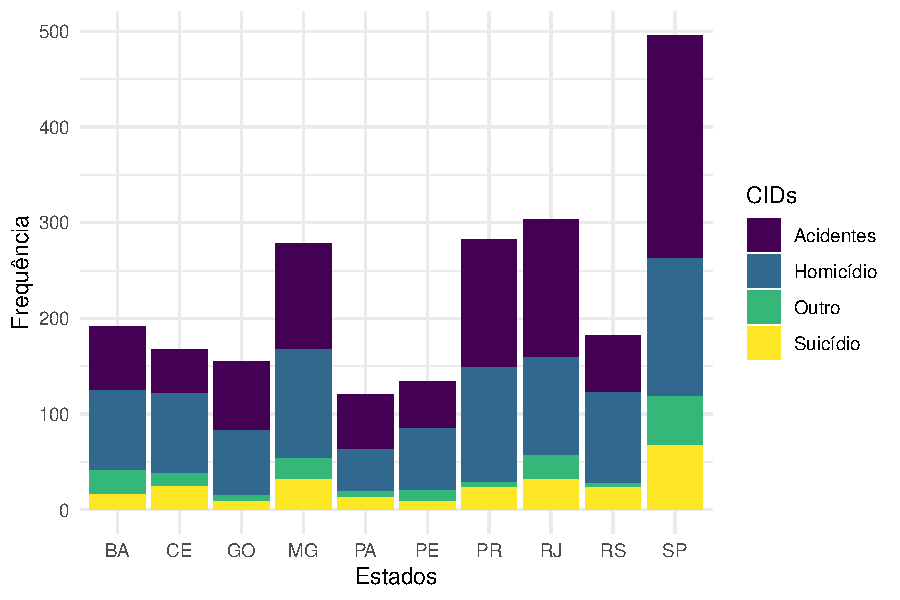
\includegraphics{RelatorioV03_files/figure-latex/unnamed-chunk-13-1.pdf}
\caption{Estados por Número de CID`s}
\end{figure}

De forma a verificar a incidência do nível de mortalidade geral e
separado por causa é feito uma análise usando como valor ``Taxa'' a
razão entre o número de casos de óbito e número de nascidos como
apresentado na Figura 6 e Figura 7, essa mesma \emph{Taxa} será
considerada em todos os gráficos de mapa apresentados, para casos de
causas específicas será considerada a razão entre o número de casos da
causa pelo número de nascidos totais.

\begin{figure}
\centering
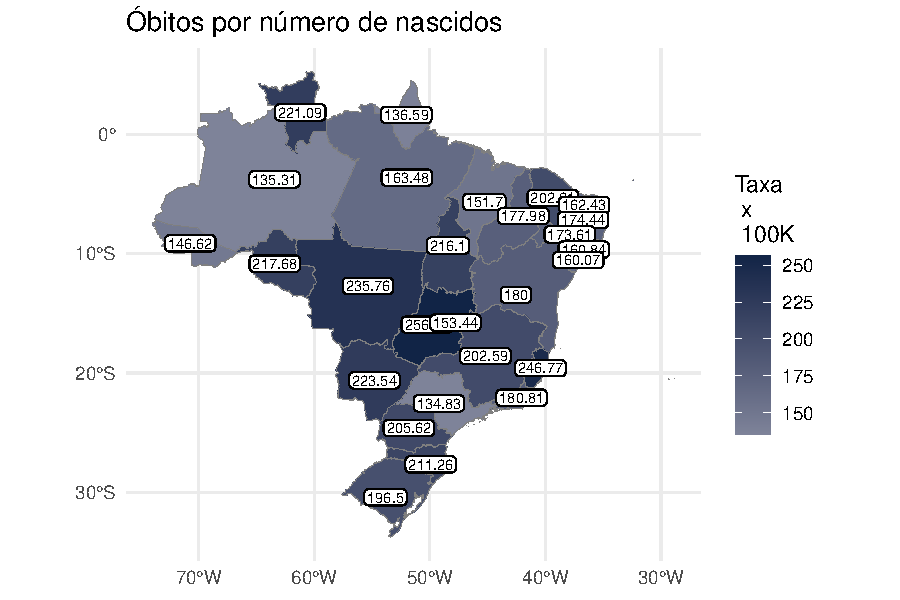
\includegraphics{RelatorioV03_files/figure-latex/unnamed-chunk-15-1.pdf}
\caption{Dados Gerais}
\end{figure}

\begin{figure}
\centering
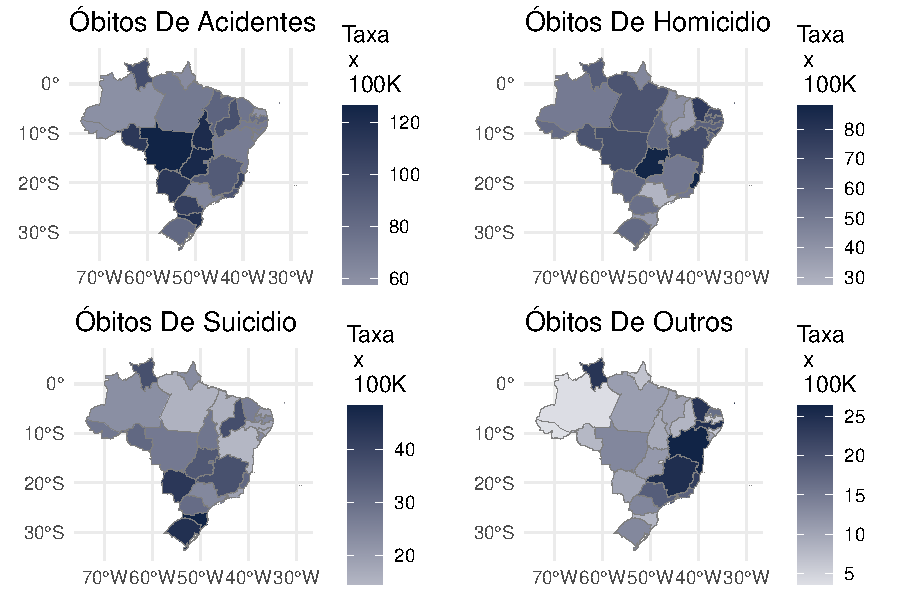
\includegraphics{RelatorioV03_files/figure-latex/unnamed-chunk-16-1.pdf}
\caption{Separados por CID}
\end{figure}

\hypertarget{gestantes-e-puuxe9rperas.-1}{%
\subsubsection{Gestantes e
Puérperas.}\label{gestantes-e-puuxe9rperas.-1}}

Apóes a visulização dos dados gerais, é apresentado pela Figura 8 o
número de casos observados para o grupo em questão para os 10 estados de
residência com maior número de incidência separando por CID.

\begin{figure}
\centering
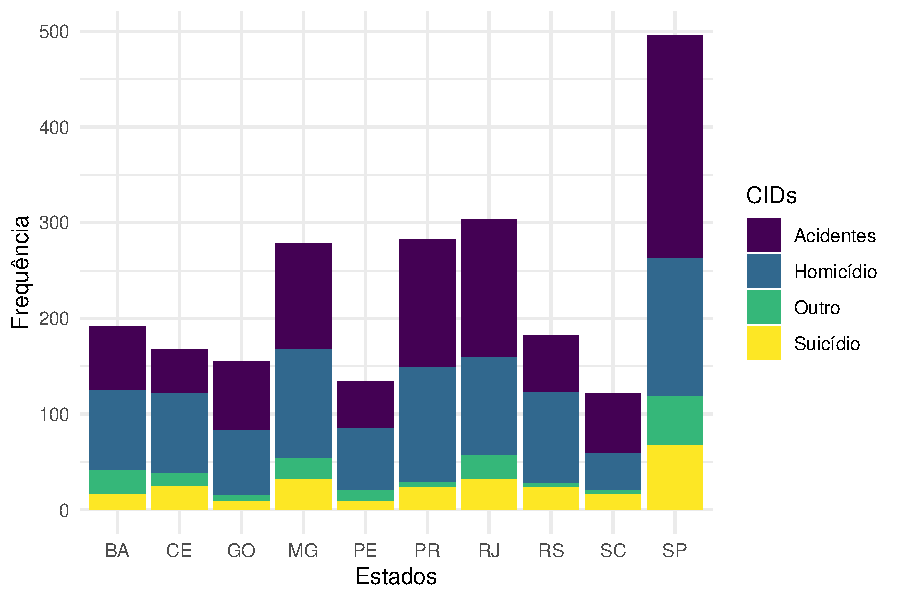
\includegraphics{RelatorioV03_files/figure-latex/unnamed-chunk-17-1.pdf}
\caption{Estados por Número de CID`s para Gestantes e Puérperas}
\end{figure}

Agora seguindo com a Figuras 9 verificamos o nível de mortalidade usando
o mesmo calculo descrito anteriormente (Número de Casos/Número de
Nascidos), para o grupo em questão.

\begin{figure}
\centering
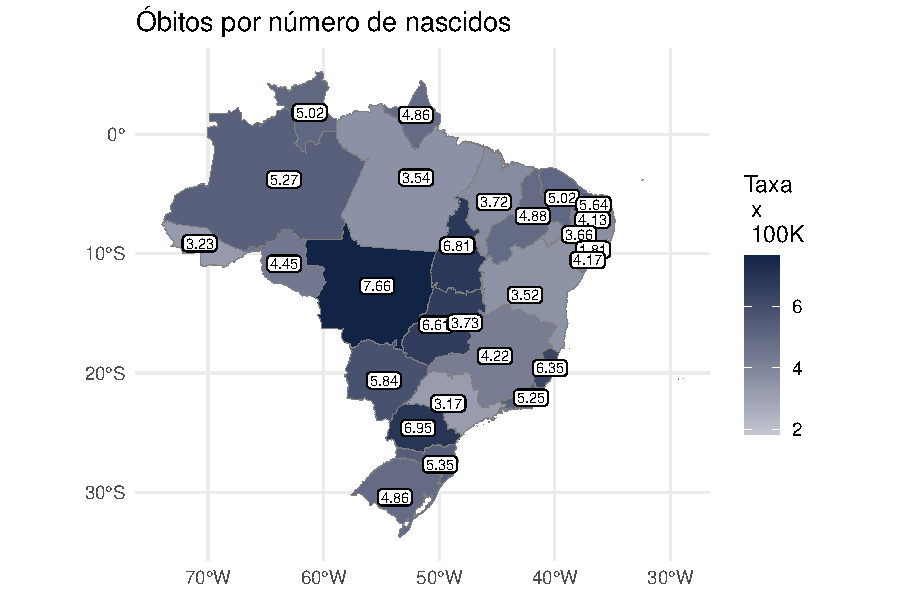
\includegraphics{RelatorioV03_files/figure-latex/unnamed-chunk-18-1.pdf}
\caption{Gestantes e Puérperas}
\end{figure}

Na Figura 10 podemos ver esses dados serapados por causas de morte.

\begin{figure}
\centering
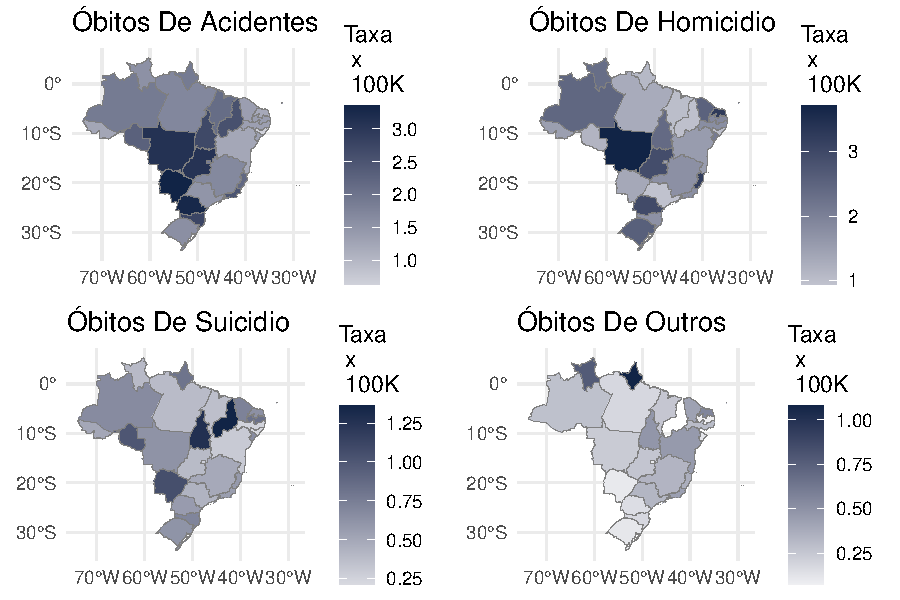
\includegraphics{RelatorioV03_files/figure-latex/unnamed-chunk-19-1.pdf}
\caption{Gestantes e Puérperas separados por CID}
\end{figure}

\hypertarget{mulheres-em-peruxedodo-fuxe9rtil.-2}{%
\subsubsection{Mulheres em Período
Fértil.}\label{mulheres-em-peruxedodo-fuxe9rtil.-2}}

Bem como feito até aqui, na Figura 11 vemos o número de casos para o
grupo de mulheres em período fértil separado por CID.

\begin{figure}
\centering
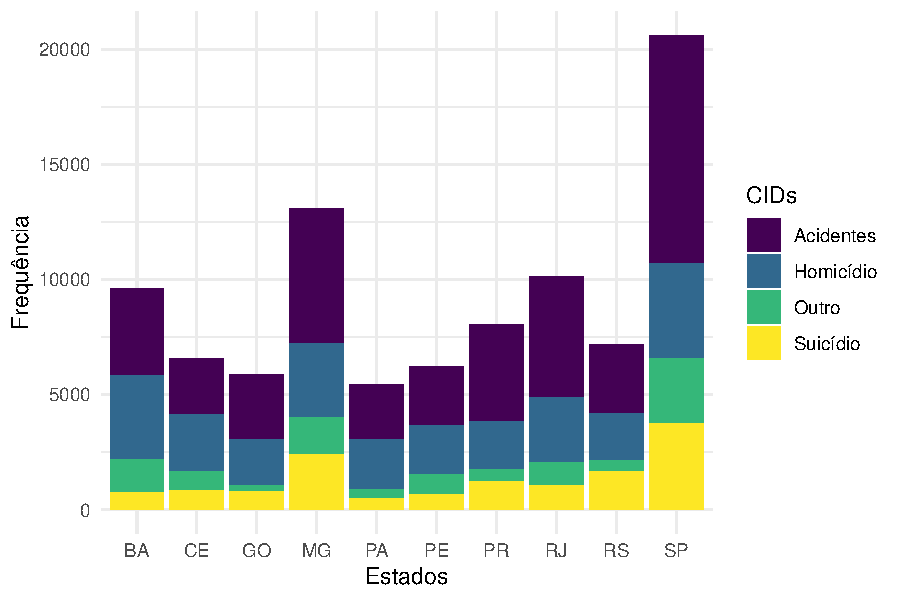
\includegraphics{RelatorioV03_files/figure-latex/unnamed-chunk-20-1.pdf}
\caption{Estados por Número de CID`s para Mulheres em Período Fértil}
\end{figure}

Seguindo com as Figuras 12 e 13 vemos a taxa de casos para o grupo em
questão.

\begin{figure}
\centering
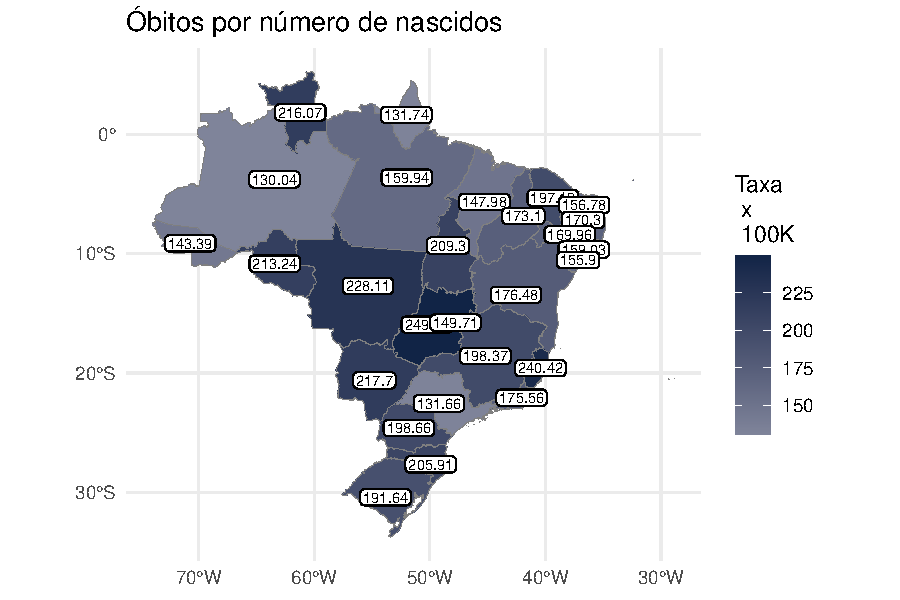
\includegraphics{RelatorioV03_files/figure-latex/unnamed-chunk-21-1.pdf}
\caption{Mulheres em Periodo Fértil}
\end{figure}

\begin{figure}
\centering
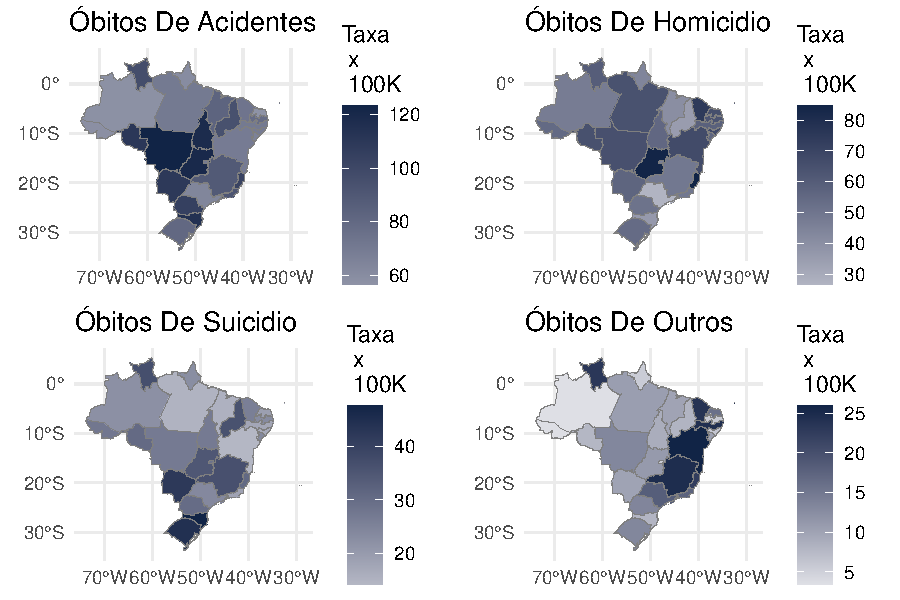
\includegraphics{RelatorioV03_files/figure-latex/unnamed-chunk-22-1.pdf}
\caption{Mulheres em período fértil separados por CID}
\end{figure}

As porcentagens não foram apresentadas nos submapas de Morte por CID em
virtude de seu baixo valor.

\hypertarget{algumas-conclusuxf5es}{%
\subsection{Algumas Conclusões}\label{algumas-conclusuxf5es}}

Com base na análise estatística dos dados, podemos chegar a algumas
conclusões importantes:

\begin{itemize}
\item
  Tendência geral de mortalidade: Observamos que os dados de mortalidade
  apresentaram uma tendência decrescente desde 2012, indicando uma
  melhoria geral na saúde e nas condições de vida. No entanto, foi
  observado um leve aumento de mortalidade de 2019 para 2020. É
  importante ressaltar que não possuímos dados relacionados à pandemia
  de COVID-19, o que poderia influenciar significativamente os
  resultados.
\item
  Diferenças na mortalidade entre grupos: Identificamos que alguns
  grupos apresentaram taxas de mortalidade mais elevadas em comparação a
  outros. Isso sugere a existência de fatores de risco específicos ou
  condições desfavoráveis que afetam esses grupos de forma
  desproporcional. Essas diferenças devem ser investigadas mais a fundo
  para identificar as possíveis causas e desenvolver estratégias de
  intervenção adequadas.
\item
  Período gestacional mais vulnerável: A análise revelou que
  determinados períodos gestacionais estão associados a maiores índices
  de homicídio e suicídio. Isso indica a necessidade de atenção e
  suporte especializado durante esses períodos para prevenir tais
  ocorrências. Além disso, por meio de testes bilaterais, identificamos
  quais grupos específicos apresentam diferenças significativas em
  relação aos índices de homicídio e suicídio.
\item
  Dependência das variáveis demográficas: Foi constatado que as
  variáveis demográficas, como sexo, faixa etária, escolaridade, estado
  civil e raça/cor, estão relacionadas de forma dependente aos casos de
  homicídio e suicídio. Isso sugere a influência dessas variáveis na
  ocorrência desses eventos e a importância de considerá-las ao
  desenvolver estratégias de prevenção e intervenção.
\item
  Diferenças nas Causas CID entre os estados: Também identificamos
  diferenças nas causas de morte (CID) entre os estados. Isso ressalta a
  importância de análises regionais para entender melhor os padrões de
  mortalidade e direcionar políticas de saúde específicas para cada
  localidade.
\end{itemize}

\end{document}
